%%%%%%%%%%%%%%%%%%%%%%%%%%%%%%%%%%%%%%%%%
% Beamer Presentation
% LaTeX Template
% Version 2.0 (March 8, 2022)
%
% This template originates from:
% https://www.LaTeXTemplates.com
%
% Author:
% Vel (vel@latextemplates.com)
%
% License:
% CC BY-NC-SA 4.0 (https://creativecommons.org/licenses/by-nc-sa/4.0/)
%
%%%%%%%%%%%%%%%%%%%%%%%%%%%%%%%%%%%%%%%%%

%%%%%%%%%%%%%%%%%%%%%%%%%%%%%%%%%%%%%%%%%
% This presentation template is an adaptation of the template mentioned above. It has been created by Giovanni Spadaro and it is available on GitHub (https://github.com/Giovo17/presentation-template-unict-lm-data).
%%%%%%%%%%%%%%%%%%%%%%%%%%%%%%%%%%%%%%%%%

%----------------------------------------------------------------------------------------
%	PACKAGES AND OTHER DOCUMENT CONFIGURATIONS
%----------------------------------------------------------------------------------------

\documentclass[
	11pt, % Set the default font size, options include: 8pt, 9pt, 10pt, 11pt, 12pt, 14pt, 17pt, 20pt
	%t, % Uncomment to vertically align all slide content to the top of the slide, rather than the default centered
	%aspectratio=169, % Uncomment to set the aspect ratio to a 16:9 ratio which matches the aspect ratio of 1080p and 4K screens and projectors
]{beamer}

\graphicspath{{img/}} % Specifies where to look for included images (trailing slash required)

\usepackage{booktabs} % Allows the use of \toprule, \midrule and \bottomrule for better rules in tables

%----------------------------------------------------------------------------------------
%	SELECT LAYOUT THEME
%----------------------------------------------------------------------------------------

% Beamer comes with a number of default layout themes which change the colors and layouts of slides. Below is a list of all themes available, uncomment each in turn to see what they look like.

%\usetheme{default}
%\usetheme{AnnArbor}
%\usetheme{Antibes}
%\usetheme{Bergen}
%\usetheme{Berkeley}
%\usetheme{Berlin}
\usetheme{Boadilla}
%\usetheme{CambridgeUS}
%\usetheme{Copenhagen}
%\usetheme{Darmstadt}
%\usetheme{Dresden}
%\usetheme{Frankfurt}
%\usetheme{Goettingen}
%\usetheme{Hannover}
%\usetheme{Ilmenau}
%\usetheme{JuanLesPins}
%\usetheme{Luebeck}
%\usetheme{Madrid}
%\usetheme{Malmoe}
%\usetheme{Marburg}
%\usetheme{Montpellier}
%\usetheme{PaloAlto}
%\usetheme{Pittsburgh}
%\usetheme{Rochester}
%\usetheme{Singapore}
%\usetheme{Szeged}
%\usetheme{Warsaw}

%----------------------------------------------------------------------------------------
%	SELECT COLOR THEME
%----------------------------------------------------------------------------------------

% Beamer comes with a number of color themes that can be applied to any layout theme to change its colors. Uncomment each of these in turn to see how they change the colors of your selected layout theme.

%\usecolortheme{albatross}
%\usecolortheme{beaver}   % red
%\usecolortheme{beetle}
%\usecolortheme{crane}   % yellow
%\usecolortheme{dolphin}  % purple
%\usecolortheme{dove}   % white
%\usecolortheme{fly}   % grey
%\usecolortheme{lily}   % purple
%\usecolortheme{monarca}   % yellow background and black
%\usecolortheme{seagull}
%\usecolortheme{seahorse}
%\usecolortheme{spruce}   % green
\usecolortheme{whale}
%\usecolortheme{wolverine}

%----------------------------------------------------------------------------------------
%	SELECT FONT THEME & FONTS
%----------------------------------------------------------------------------------------

% Beamer comes with several font themes to easily change the fonts used in various parts of the presentation. Review the comments beside each one to decide if you would like to use it. Note that additional options can be specified for several of these font themes, consult the beamer documentation for more information.

\usefonttheme{default} % Typeset using the default sans serif font
%\usefonttheme{serif} % Typeset using the default serif font (make sure a sans font isn't being set as the default font if you use this option!)
%\usefonttheme{structurebold} % Typeset important structure text (titles, headlines, footlines, sidebar, etc) in bold
%\usefonttheme{structureitalicserif} % Typeset important structure text (titles, headlines, footlines, sidebar, etc) in italic serif
%\usefonttheme{structuresmallcapsserif} % Typeset important structure text (titles, headlines, footlines, sidebar, etc) in small caps serif

%------------------------------------------------

%\usepackage{mathptmx} % Use the Times font for serif text
\usepackage{palatino} % Use the Palatino font for serif text

%\usepackage{helvet} % Use the Helvetica font for sans serif text
\usepackage[default]{opensans} % Use the Open Sans font for sans serif text
%\usepackage[default]{FiraSans} % Use the Fira Sans font for sans serif text
%\usepackage[default]{lato} % Use the Lato font for sans serif text

%----------------------------------------------------------------------------------------
%	SELECT INNER THEME
%----------------------------------------------------------------------------------------

% Inner themes change the styling of internal slide elements, for example: bullet points, blocks, bibliography entries, title pages, theorems, etc. Uncomment each theme in turn to see what changes it makes to your presentation.

%\useinnertheme{default}
\useinnertheme{circles}
%\useinnertheme{rectangles}
%\useinnertheme{rounded}
%\useinnertheme{inmargin}

%----------------------------------------------------------------------------------------
%	SELECT OUTER THEME
%----------------------------------------------------------------------------------------

% Outer themes change the overall layout of slides, such as: header and footer lines, sidebars and slide titles. Uncomment each theme in turn to see what changes it makes to your presentation.

%\useoutertheme{default}
%\useoutertheme{infolines}
\useoutertheme{miniframes}
%\useoutertheme{smoothbars}
%\useoutertheme{sidebar}
%\useoutertheme{split}
%\useoutertheme{shadow}
%\useoutertheme{tree}
%\useoutertheme{smoothtree}

%\setbeamertemplate{footline} % Uncomment this line to remove the footer line in all slides
%\setbeamertemplate{footline}[page number] % Uncomment this line to replace the footer line in all slides with a simple slide count

%\setbeamertemplate{navigation symbols}{} % Uncomment this line to remove the navigation symbols from the bottom of all slides

%----------------------------------------------------------------------------------------
%	PRESENTATION INFORMATION
%----------------------------------------------------------------------------------------

\title[FoundationDB]{FoundationDB:
A Distributed Key-Value Store} % The short title in the optional parameter appears at the bottom of every slide, the full title in the main parameter is only on the title page

%\subtitle{Optional Subtitle} % Presentation subtitle, remove this command if a subtitle isn't required

\author[Ciccarello]{Andrea Ciccarello} % Presenter name(s), the optional parameter can contain a shortened version to appear on the bottom of every slide, while the main parameter will appear on the title slide

\institute[UNIPR]{Università degli studi di Parma} % Your institution, the optional parameter can be used for the institution shorthand and will appear on the bottom of every slide after author names, while the required parameter is used on the title slide and can include your email address or additional information on separate lines

\date[2024]{May-June 2024} % Presentation date or conference/meeting name, the optional parameter can contain a shortened version to appear on the bottom of every slide, while the required parameter value is output to the title slide

%----------------------------------------------------------------------------------------

\begin{document}

%----------------------------------------------------------------------------------------
%	TITLE SLIDE
%----------------------------------------------------------------------------------------

\begin{frame}

        \begin{figure}
		
\includegraphics[width=0.25\linewidth]{img/logo-unipr/Logo unipr.png}
	\end{figure}
 
	\titlepage % Output the title slide, automatically created using the text entered in the PRESENTATION INFORMATION block above
\end{frame}

%----------------------------------------------------------------------------------------
%	TABLE OF CONTENTS SLIDE
%----------------------------------------------------------------------------------------

% The table of contents outputs the sections and subsections that appear in your presentation, specified with the standard \section and \subsection commands. You may either display all sections and subsections on one slide with \tableofcontents, or display each section at a time on subsequent slides with \tableofcontents[pausesections]. The latter is useful if you want to step through each section and mention what you will discuss.

\begin{frame}
	\frametitle{Presentation Overview} % Slide title, remove this command for no title
	
	\tableofcontents % Output the table of contents (all sections on one slide)
	%\tableofcontents[pausesections] % Output the table of contents (break sections up across separate slides)
\end{frame}

%----------------------------------------------------------------------------------------
%	PRESENTATION BODY SLIDES
%----------------------------------------------------------------------------------------



\section{Introduction} % Sections are added in order to organize your presentation into discrete blocks, all sections and subsections are automatically output to the table of contents as an overview of the talk but NOT output in the presentation as separate slides

%------------------------------------------------

\begin{frame}
\frametitle{FoundationDB}

\begin{figure}
    \centering
    
\includegraphics[width=0.5\textwidth]{img/1-Introduction/foundationBD-logo.png}
    
\end{figure}

\textbf{FoundationDB}FoundationDB is an open-source transactional key-value store created by Apple in 2009. It combine \textbf{flexibility} and \textbf{scalability} of \textbf{NoSQL} architectures with the power of \textbf{ACID transactions}.
	
\end{frame}

%------------------------------------------------

\begin{frame}
	\frametitle{FDB Key features}

Key features:
\begin{itemize}
    \item NoSQL
    \item Ordered key-value pair.
    \item Strictly serializable transactions
    \item ACID transactions
    \item Designed around Core-Layer philosophy 
    
\end{itemize}

\end{frame}
%------------------------------------------------
\begin{frame}
	\frametitle{CAP trade off}

A trade off exists between consistency, availability, and
partition tolerance
\begin{itemize}
    \item Consistency: A read sees all previously completed writes
    \item Availability: Reads and writes always succeed
    \item Partition tolerance: Guaranteed properties are maintained even when network failures prevent some machines from communicating with others.
    
\end{itemize}
FoundationBD satisfied \textbf{Consistency} and \textbf{Partition Tolerance} 

\end{frame}
%------------------------------------------------
\begin{frame}
	\frametitle{CAP Theorem Examples}

\begin{figure}[h]
    \centering
    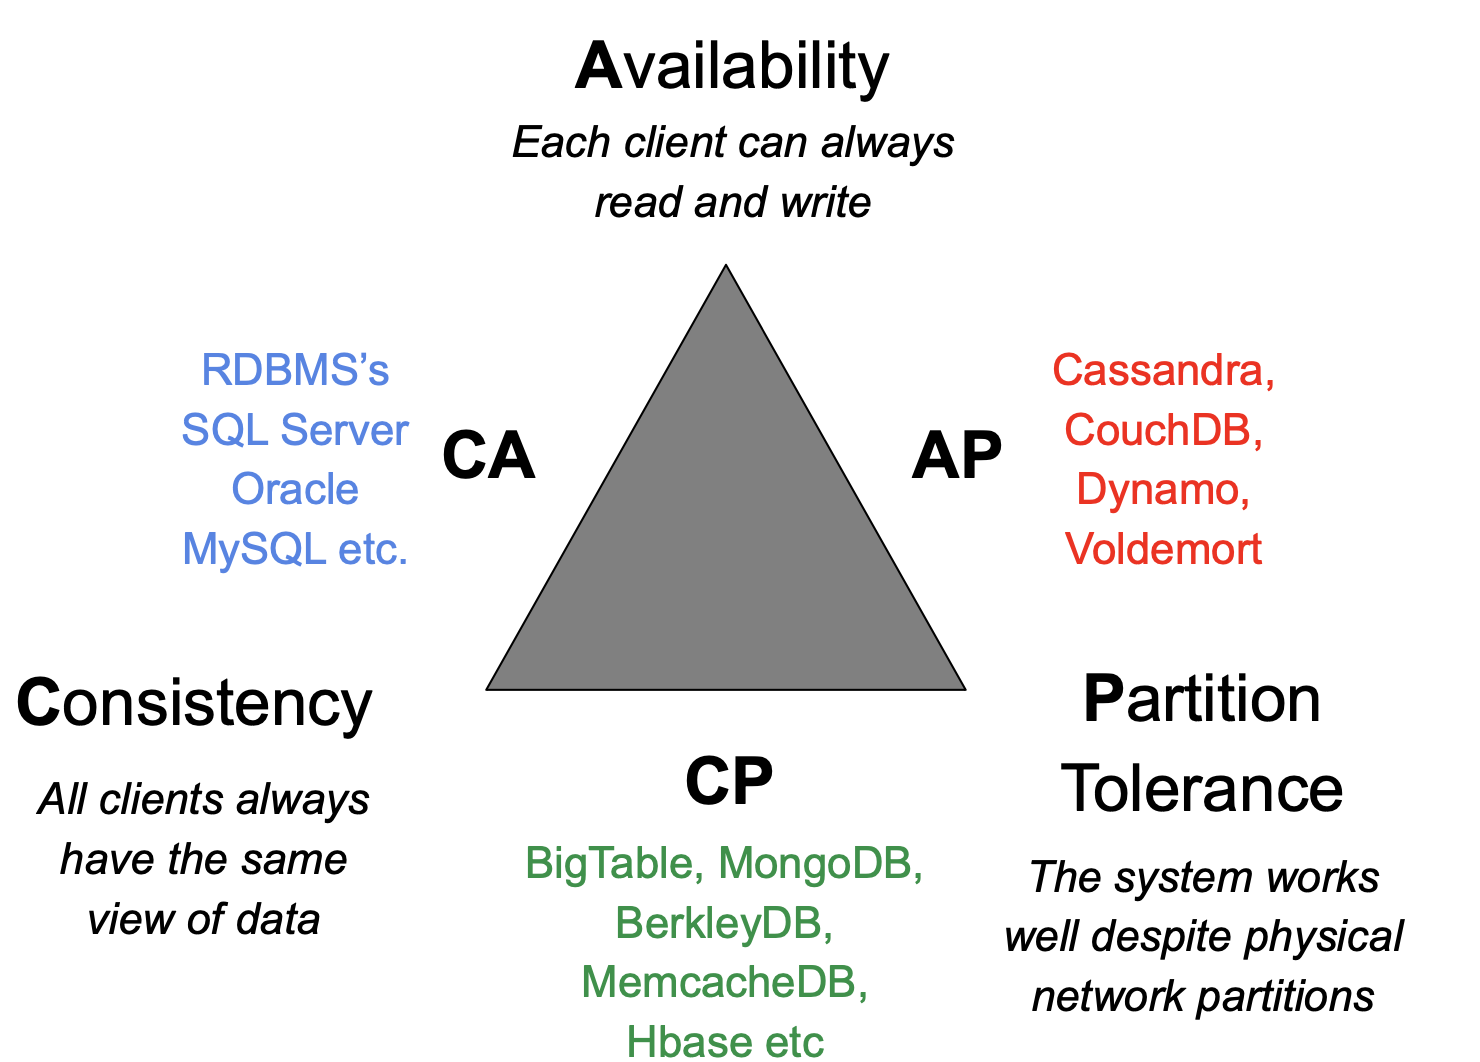
\includegraphics[width=0.7\textwidth]{img/1-Introduction/CAP theorem.png}
    \caption{CAP Theorem (or triangle)}
\end{figure}

\end{frame}

%------------------------------------------------

\begin{frame}
	\frametitle{Consistency over Availability}

 Availability in the CAP sense means that all nodes remain able to read and write even when partitioned. A system that keeps some, but not all, of its nodes able to read and write is not Available in the CAP sense, even if it remains available to clients and satisfies its SLAs for high availability.
\vspace{0.5cm}

As any ACID database must, during a network partition, FoundationDB chooses \textbf{Consistency over Availability}. 

\end{frame}

%------------------------------------------------

\begin{frame}
	\frametitle{FoundationDB approach}
Most database: 
    \begin{itemize}
        \item Storage engine
        \item Data model
        \item API/Query language
    \end{itemize}

FoundationDB has a modular approach, it it provides a highly scalable storage engine with a minimal yet carefully chosen set of features.

\vspace{0.5cm}
\begin{quote}
    \textbf{\textcolor{red}{``What features could we take away? Almost everything, we decided.''}}
\end{quote}
        
\end{frame}


%------------------------------------------------

\begin{frame}
	\frametitle{Less is more: The FoundationDB way}
FoundationDB decouples its data storage technology from its data model, core ordered key-value storage technology can be efficiently adapted and remapped to a broad array of rich data models.
\vspace{0.5cm}

\begin{center}
    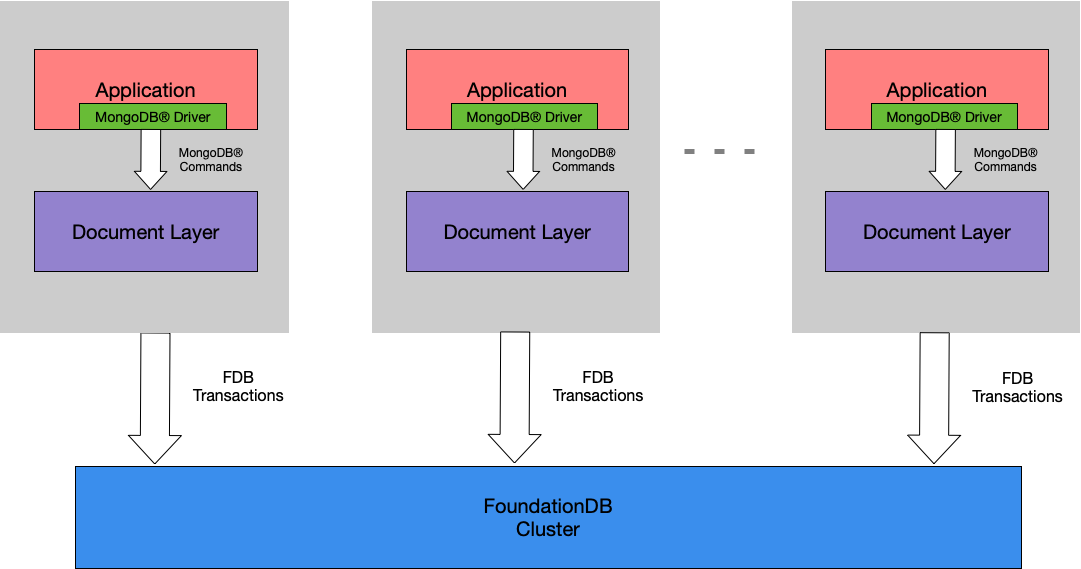
\includegraphics[width=0.6\textwidth]{img/1-Introduction/sidecar-arch.png}
\end{center}

\end{frame}

%------------------------------------------------

\begin{frame}
	\frametitle{Example: indexing}

FoundationDB’s core provides \textbf{no indexing}  (\href{https://apple.github.io/foundationdb/anti-features.html}{anti-feature}).

Instead, a layer provides indexing by storing two kinds of key-values, one for the data and one for the index.

\begin{center}
\textbf{\textcolor{red}{people/alice/eye\_color = blue}}
\end{center}

\begin{center}
\textbf{\textcolor{red}{eye\_color/blue/alice = true}}
\end{center}

ACID transactions allows to update both the data and the index in a single transaction.
\end{frame}

%------------------------------------------------

\begin{frame}
	\frametitle{Layer strategy}

FoundationBD is leaving the rest to additionals “layers”.

\vspace{0.5cm}
Examples:
\begin{itemize}
    \item \textbf{FoundationDB Record Layer}: Java Api that adds back much of what users expect from a simple relational database 
    \item CouchDB 4.0: adopt FoundationDB in 2019 as storage and replication engine.
\end{itemize}
\end{frame}


%------------------------------------------------

\begin{frame}
	\frametitle{What will be discussed in the next chapters}

    \begin{itemize}
        \item Architecture of FoundationDB
        \item Simulation and Testing of distributed system
        \item Evaluation of FoundationDB
        \item Conclusions
    \end{itemize}
        
\end{frame}

%------------------------------------------------


\section{Architecture}

%------------------------------------------------
\begin{frame}
	\frametitle{Optimistic concurrency control}
 In a system with \textbf{optimistic concurrency control}, transactions operate under the optimistic assumption that conflicts are rare. 
\vspace{0.5cm}

FoundationDB utilizes \textbf{multiversion concurrency control} as part of its optimistic approach. With MVCC, each transaction operates on a "version" of the data, reflecting a database state at a certain point in time (always a consistent view when reading).
\end{frame}

%------------------------------------------------


\begin{frame}
    \frametitle{Architecture and Transaction Processing}
    \begin{columns}
        \begin{column}{0.5\textwidth}
            \begin{itemize}
                \item \textbf{Control Plane}
                \item \textbf{Data Plane}
                \begin{itemize}
                    \item Transaction System (TS)
                    \item Log System (LS)
                    \item Storage System (SS)
                \end{itemize}
            \end{itemize}
        \end{column}
        \begin{column}{0.5\textwidth}
            \centering
            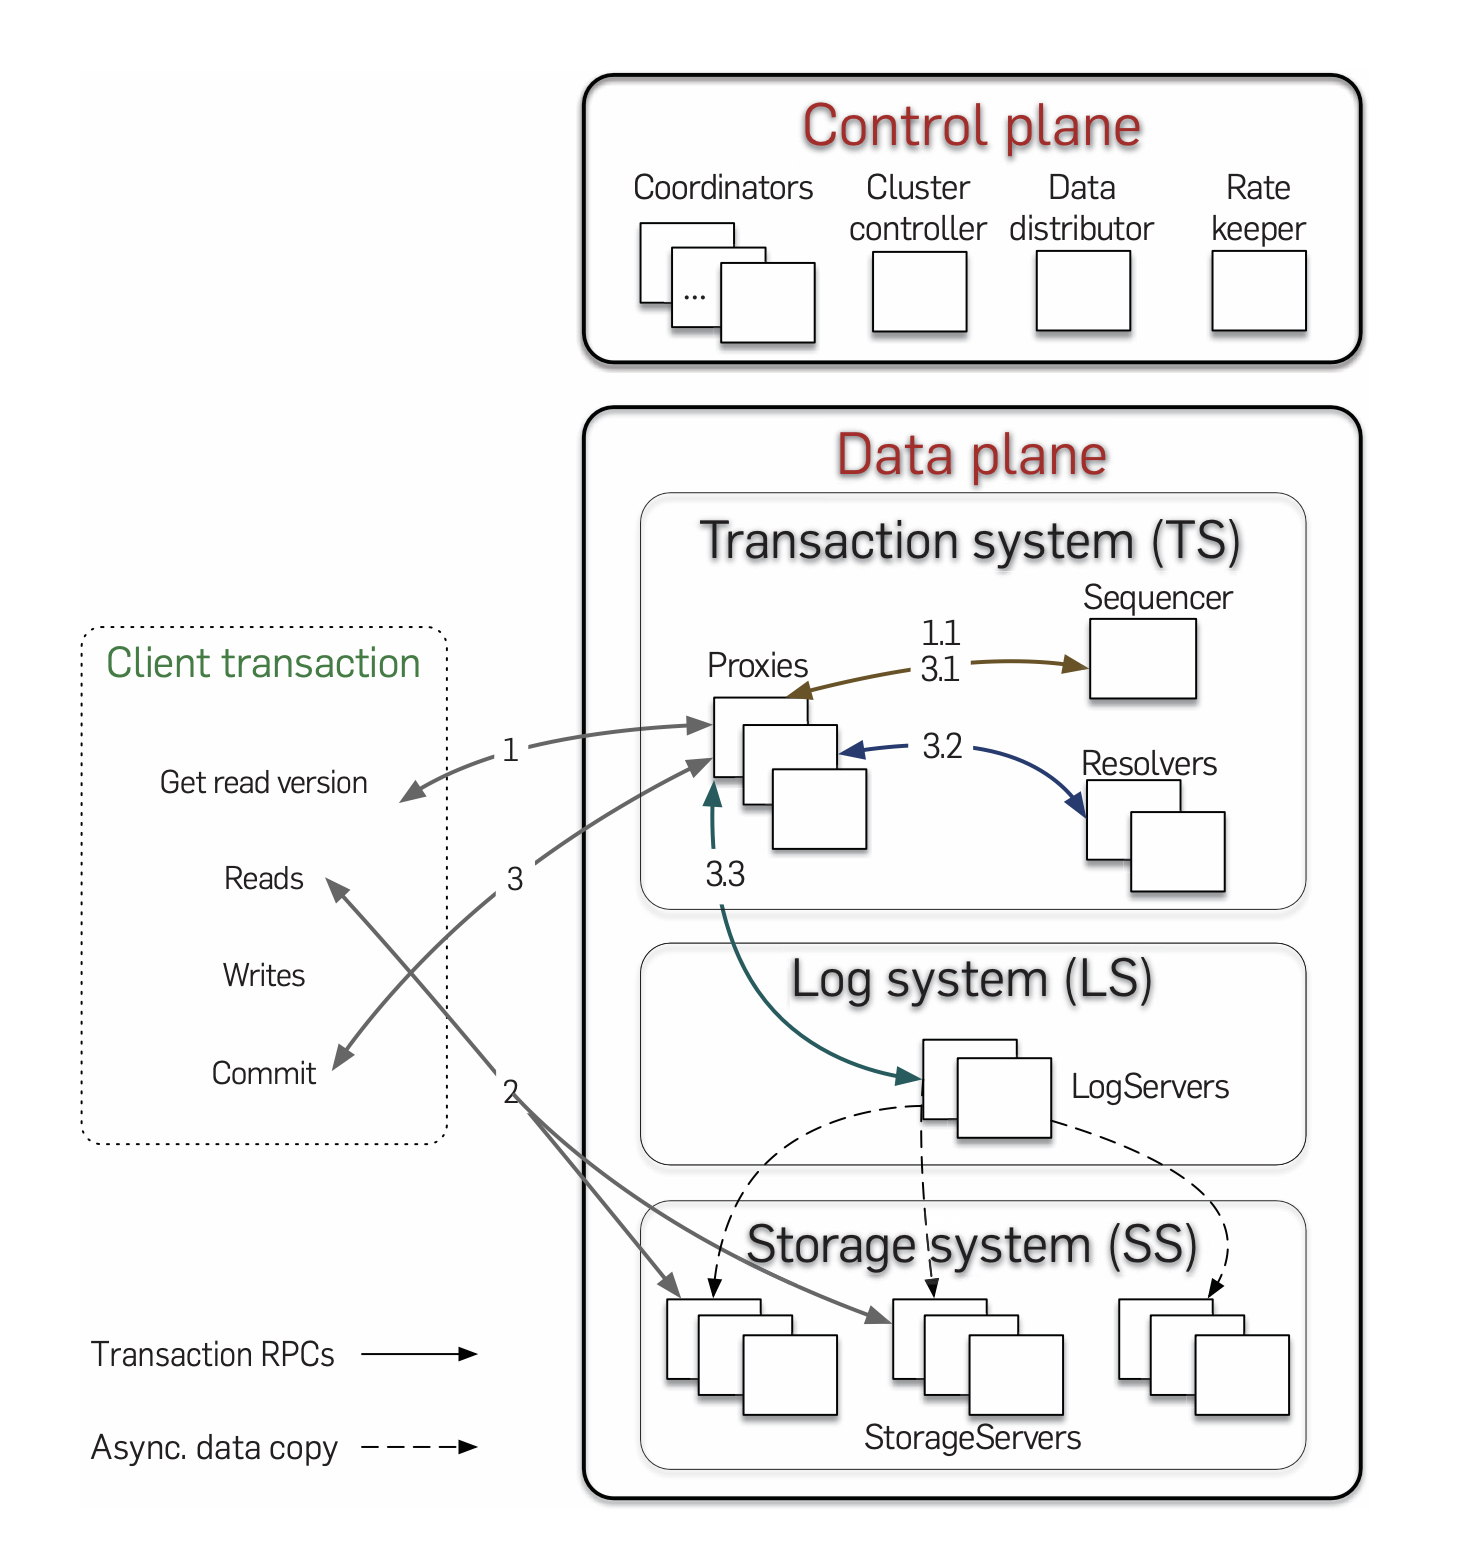
\includegraphics[width=\textwidth]{img/2-Architecture/Architecture and transaction processing.png}
        \end{column}
    \end{columns}
\end{frame}


%------------------------------------------------

% \begin{frame}
% 	\frametitle{Control plane P1}

% The control plane is responsible for persisting critical metadata of the cluster for high availability.
% \textbf{Cluster Controller} monitors all servers in the cluster and recruits 3 processes:
% \begin{itemize}
%     \item Sequencer (Data Plane)
%     \item Data Distributor
%     \item Ratekeeper
% \end{itemize}

% Coordinators form a Paxos group (consensus protocol) and elect the Cluster Controller.
% \end{frame}

%------------------------------------------------


% \begin{frame}
%     \frametitle{Control plane P2}
%     \begin{columns}
%         \begin{column}{0.5\textwidth}
%         \begin{itemize}
%         \item \textbf{Data Distributor} is responsible for monitoring failures and balancing data among Storage Servers.
%         \item \textbf{Ratekeeper} provides overload protection for the cluster.
%         \end{itemize}
        
%         \end{column}
%         \begin{column}{0.5\textwidth}
%             \centering
%             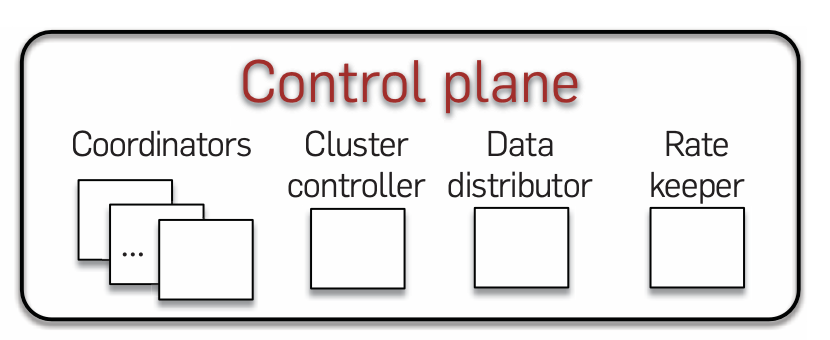
\includegraphics[width=\textwidth]{img/2-Architecture/Control plane.png}
%         \end{column}
%     \end{columns}
% \end{frame}



%------------------------------------------------


\begin{frame}
    \frametitle{Data plane: Transaction system (TS) P1}
    \begin{columns}
        \begin{column}{0.5\textwidth}
        \begin{itemize}
    \item \textbf{Sequencer}: assigns a read and a commit version to each transaction
    \item \textbf{Proxies}: offer MVCC read versions to clients and orchestrate transaction commits
    \item \textbf{Resolvers}: check for conflicts among transactions (5 seconds of history)
   \end{itemize}
        
        \end{column}
        \begin{column}{0.5\textwidth}
            \centering
            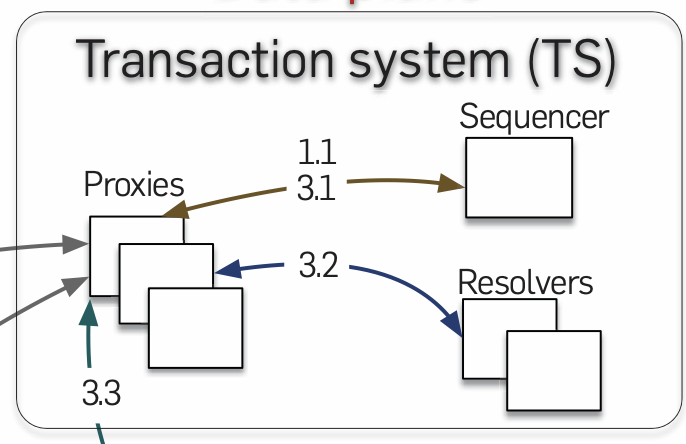
\includegraphics[width=\textwidth]{img/2-Architecture/Transaction System.png}
        \end{column}
    \end{columns}
\end{frame}

%------------------------------------------------

% \begin{frame}
% 	\frametitle{Data plane: Transaction system (TS) P2}

% FoundationDB uses \textbf{multiversion concurrency control} to provide transactionally isolated reads without locking data or blocking writes.
% \vspace{0.5cm}

% \textbf{Optimistic concurrency control} ensures that deadlocks are impossible and that slow or failing clients cannot interfere with the operation of the database.
	
% \end{frame}

% %------------------------------------------------


\begin{frame}
    \frametitle{Data plane: Log system (LS)}
    \begin{columns}
        \begin{column}{0.5\textwidth}
        \textbf{Log Servers} act as replicated, distributed persistent queues, each queue storing "Write-Ahead Log" data for a Storage Server.
        
        \end{column}
        \begin{column}{0.5\textwidth}
            \centering
            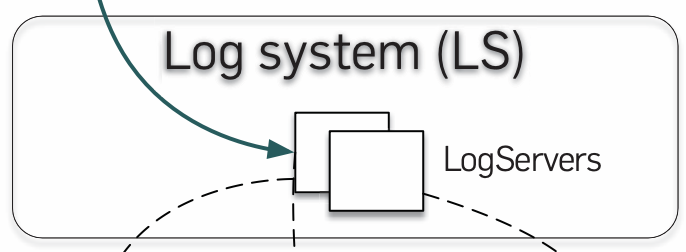
\includegraphics[width=\textwidth]{img/2-Architecture/log system.png}
        \end{column}
    \end{columns}
\end{frame}

% %------------------------------------------------


\begin{frame}
    \frametitle{Data plane: Storage system (SS)}
    \begin{columns}
        \begin{column}{0.5\textwidth}
        The Storage system consists of a number of \textbf{Storage Servers}, each
storing a set of data shards (contiguous key ranges),
and serving client reads. 
\vspace{0.5cm}

Storage Servers are the majority of processes in the system, and together they form a distributed B-tree.
        
        \end{column}
        \begin{column}{0.5\textwidth}
            \centering
            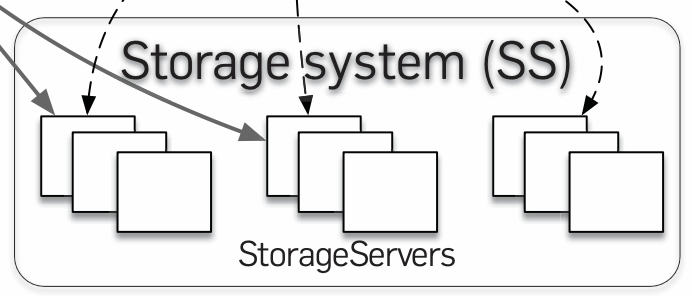
\includegraphics[width=\textwidth]{img/2-Architecture/Storage system.png}
        \end{column}
    \end{columns}
\end{frame}

% %------------------------------------------------
% \begin{frame}
% 	\frametitle{Scaling}
% Scaling is just adding processes for each role. \\

% \begin{itemize}
% \item Clients read from sharded Storage Servers, so reads scale
% linearly with the number of Storage Servers. 
% \end{itemize}

% \vspace{0.5cm}
% Coordinators and control plane's singleton processes like \textbf{Cluster Controller} and \textbf{Sequencer} only perform limited metadata operations.
	
% \end{frame}
% %------------------------------------------------

\begin{frame}
    \frametitle{Transactions: Read}
    \begin{columns}
        \begin{column}{0.5\textwidth}
            \begin{enumerate}
    \item Client $\rightarrow$ Proxies to obtain a read version (timestamp).
    \item Proxy $\rightarrow$ the Sequencer requesting a read version, that is  least as large as all previously issued transaction commit versions.
            \end{enumerate}
        \end{column}
        \begin{column}{0.5\textwidth}
            \centering
            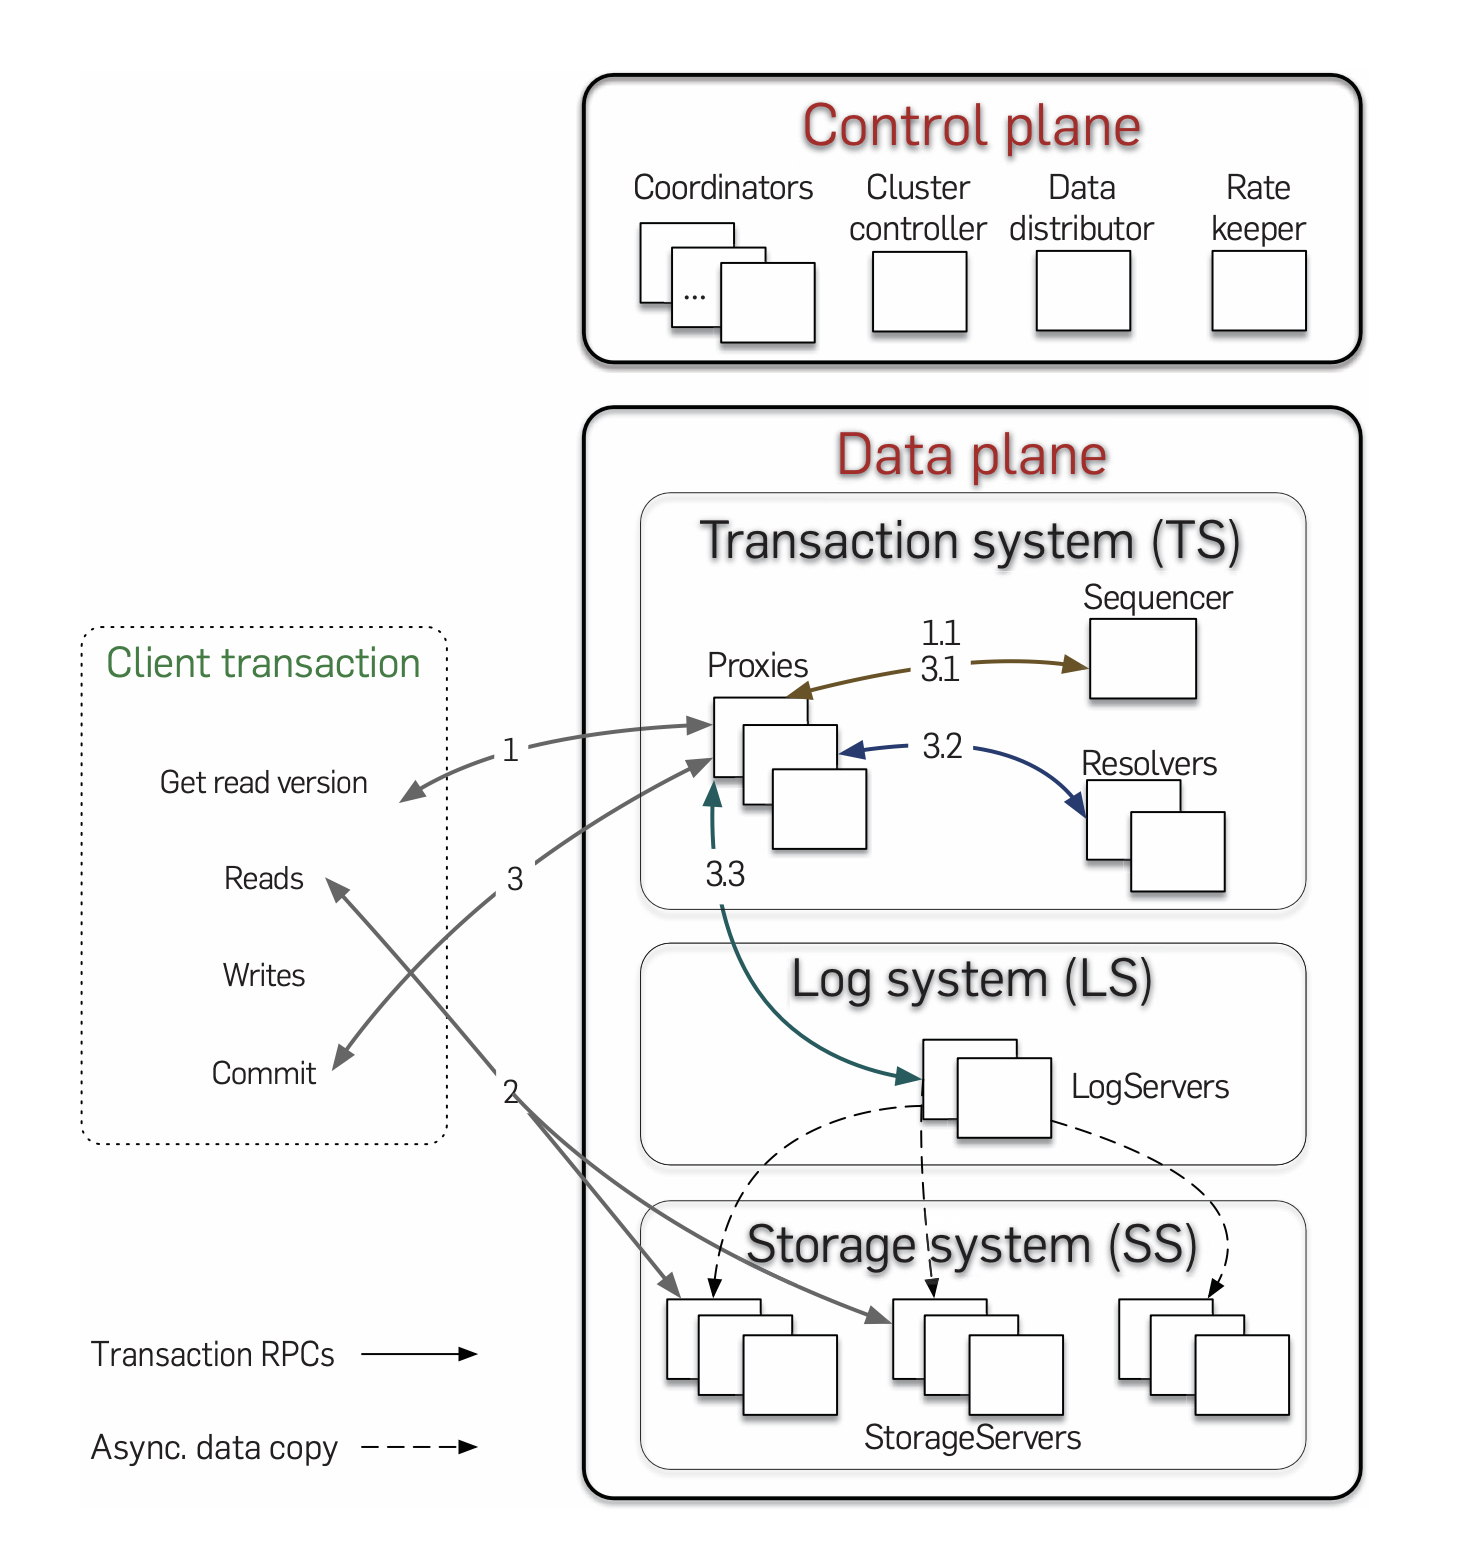
\includegraphics[width=\textwidth]{img/2-Architecture/Architecture and transaction processing.png}
        \end{column}
    \end{columns}
\end{frame}

% %------------------------------------------------

\begin{frame}
    \frametitle{Transactions: Read P2}
    \begin{columns}
        \begin{column}{0.5\textwidth}
            \begin{enumerate}
    \item Proxy $\rightarrow$ client read version.
    \item Client reads from Storage Servers.
    \item Client can cache this information for the next read if needed.
            \end{enumerate}
        \end{column}
        \begin{column}{0.5\textwidth}
            \centering
            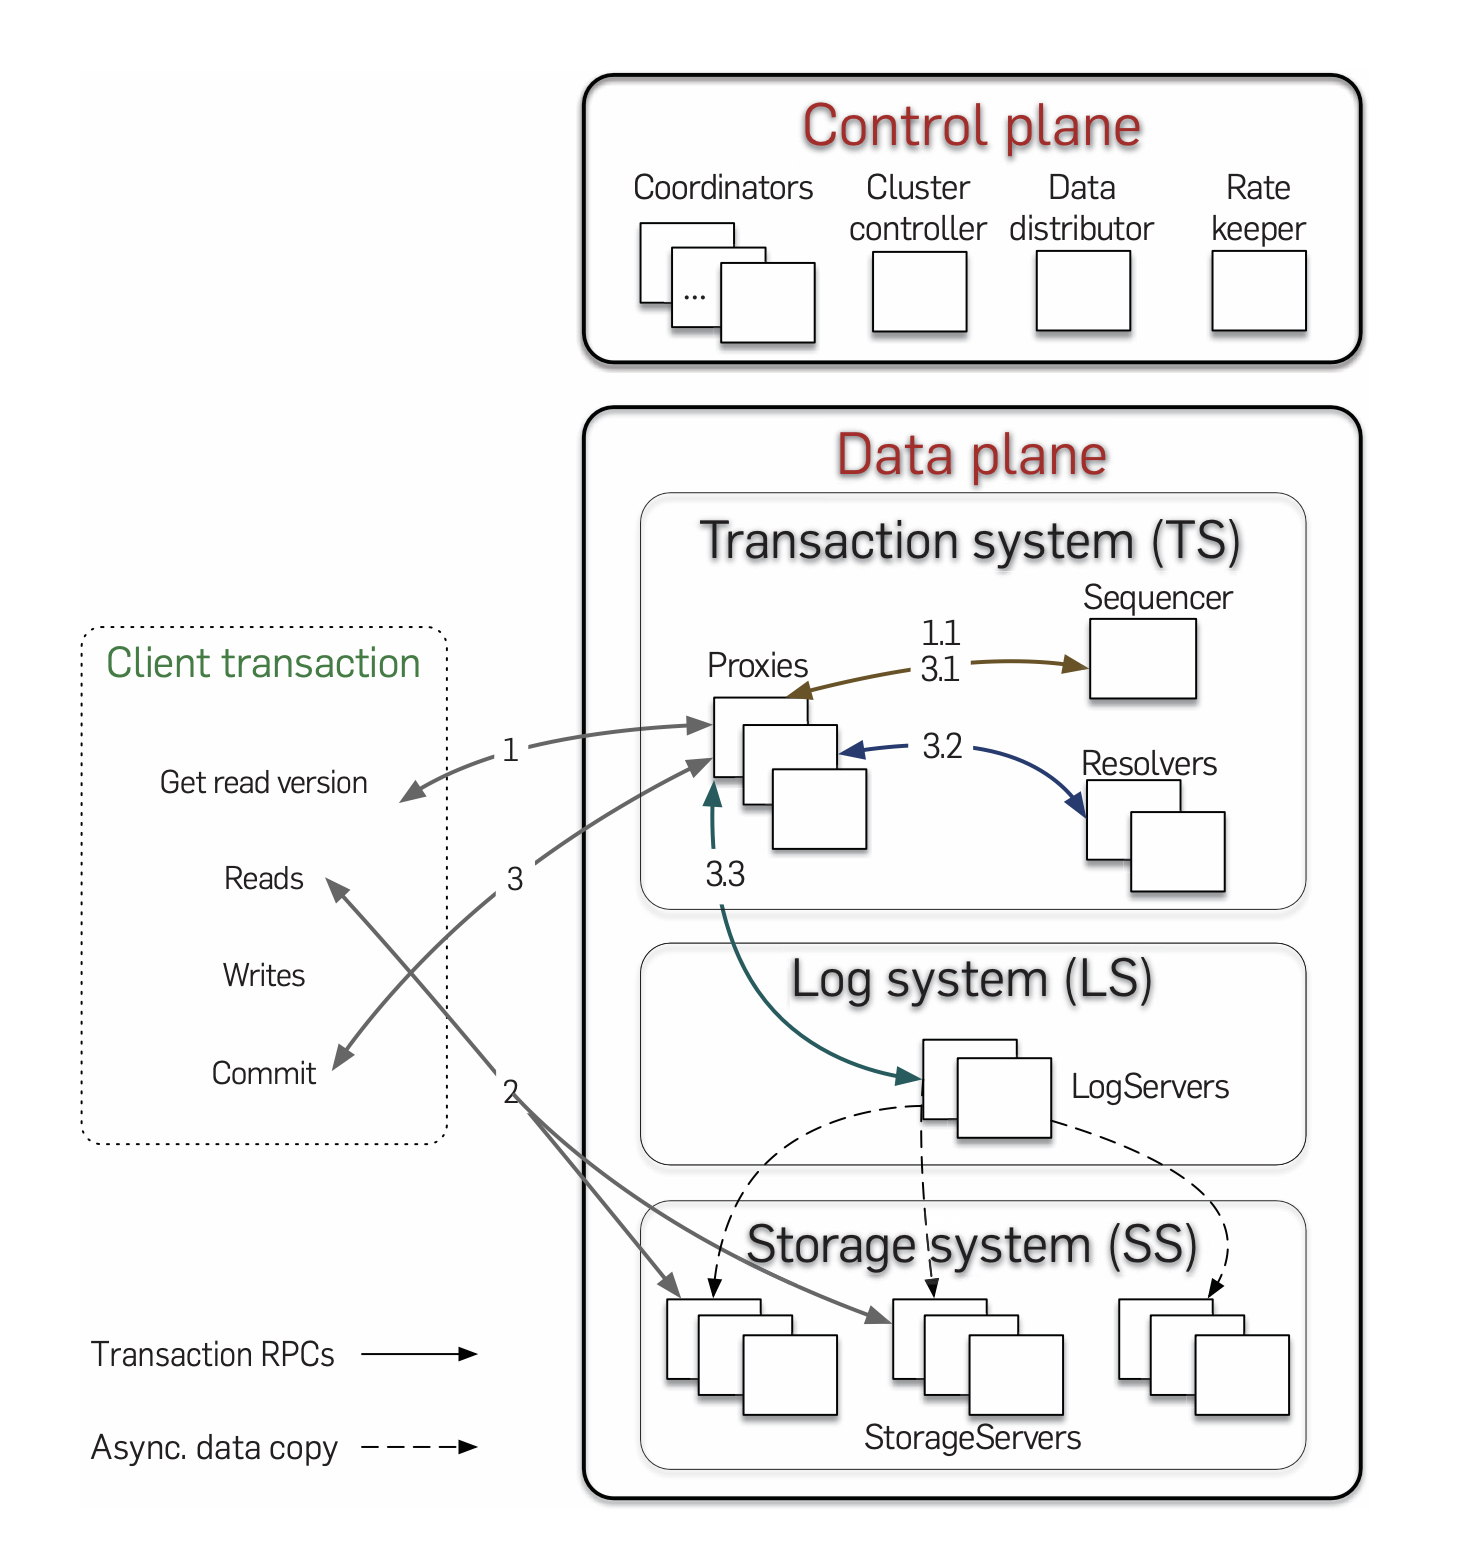
\includegraphics[width=\textwidth]{img/2-Architecture/Architecture and transaction processing.png}
        \end{column}
    \end{columns}
\end{frame}

% %------------------------------------------------

\begin{frame}
    \frametitle{Transactions: Writes}
    \begin{columns}
        \begin{column}{0.5\textwidth}
            \begin{enumerate}
                \item When the client sends the \textbf{transaction data} (read and write that you have done in the transaction) to one of the Proxies
                \item Client waits for a response (commit or abort)
            \end{enumerate}
        \end{column}
        \begin{column}{0.5\textwidth}
            \centering
            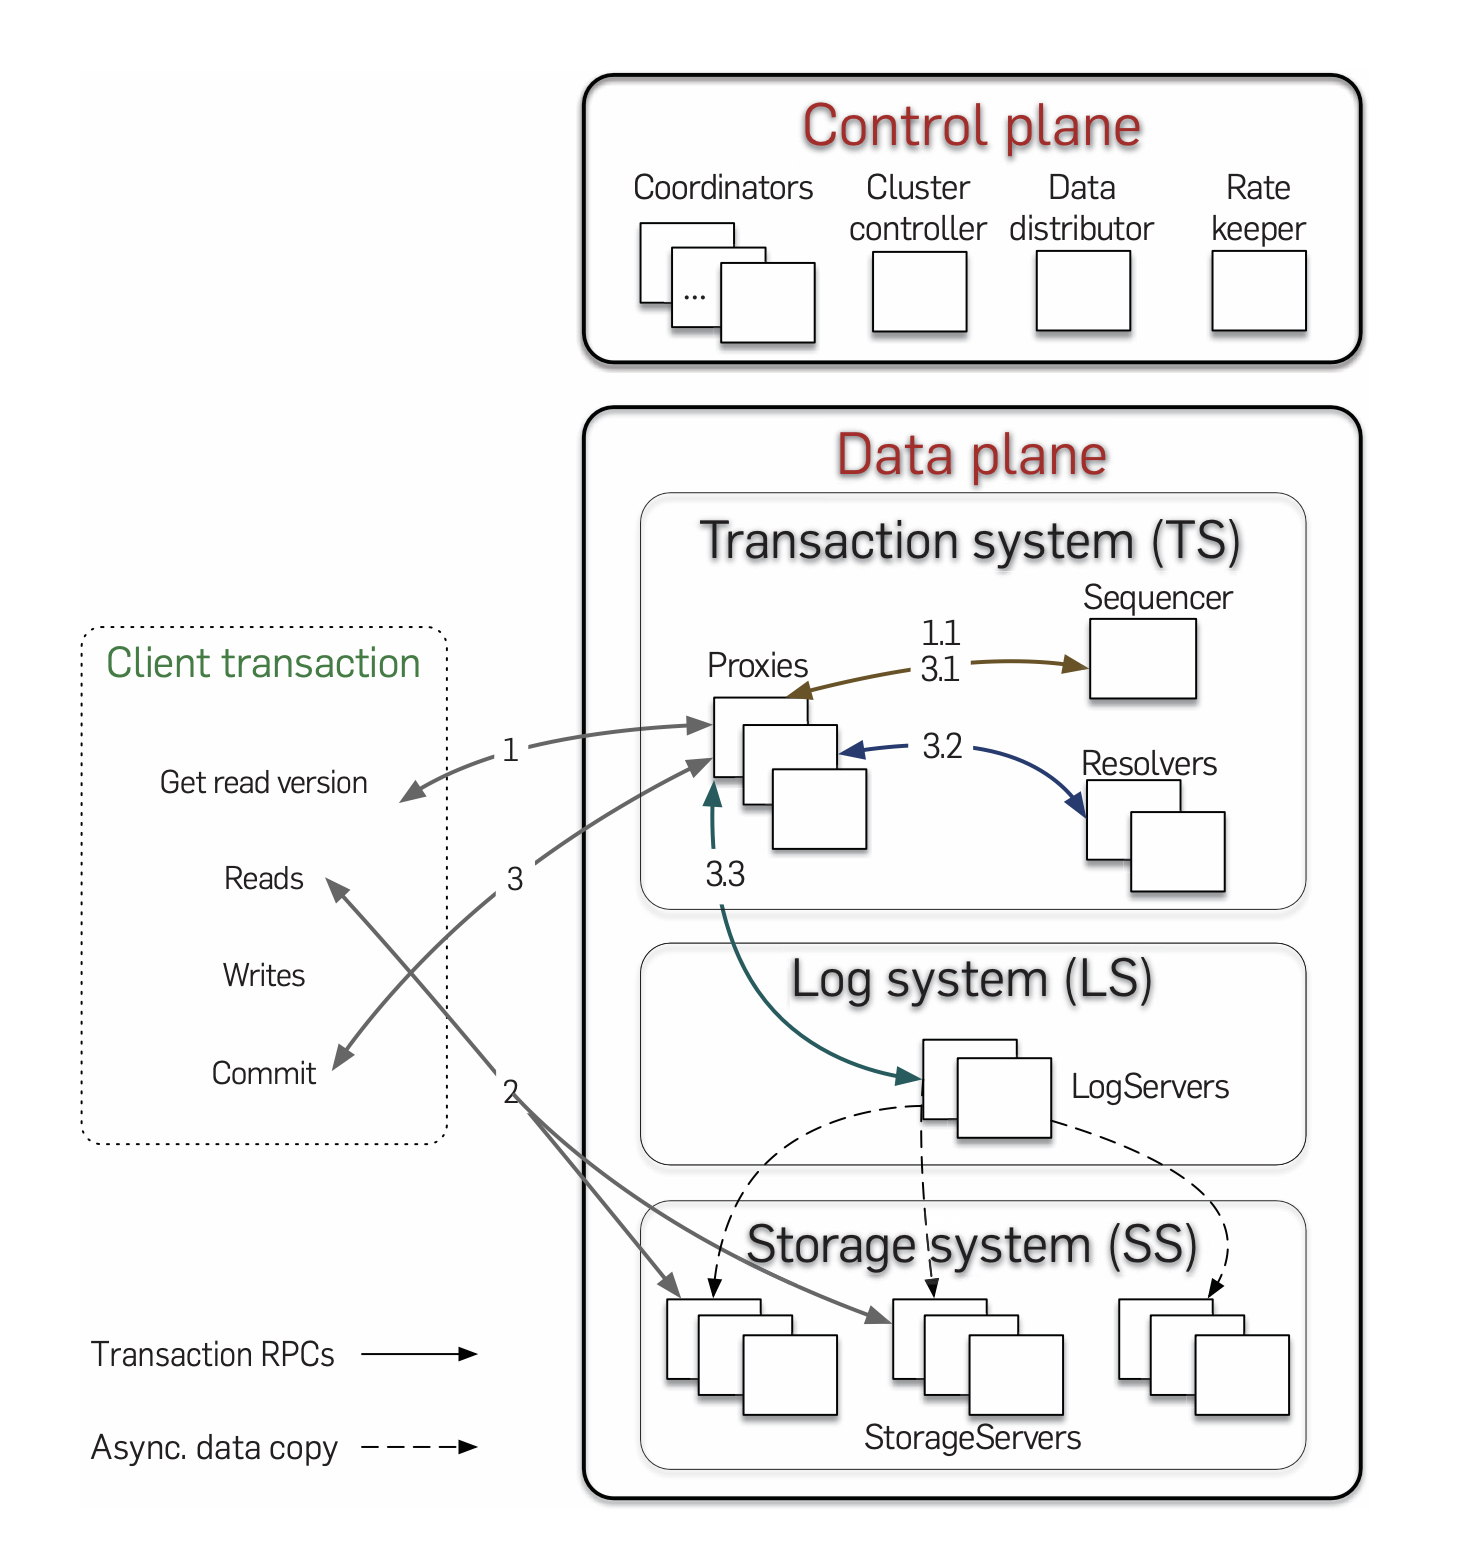
\includegraphics[width=\textwidth]{img/2-Architecture/Architecture and transaction processing.png}
        \end{column}
    \end{columns}
\end{frame}


% %------------------------------------------------
\begin{frame}
    \frametitle{Transactions: Proxy commits}
    \begin{columns}
        \begin{column}{0.5\textwidth}
            \begin{enumerate}
\item Transaction $\rightarrow$ to \textbf{Resolvers} that have to handle the OCC by checking for \b conflicts.
    \item Transaction is forwarded to a set of designated \textbf{Log Servers}.
            \end{enumerate}
        \end{column}
        \begin{column}{0.5\textwidth}
            \centering
            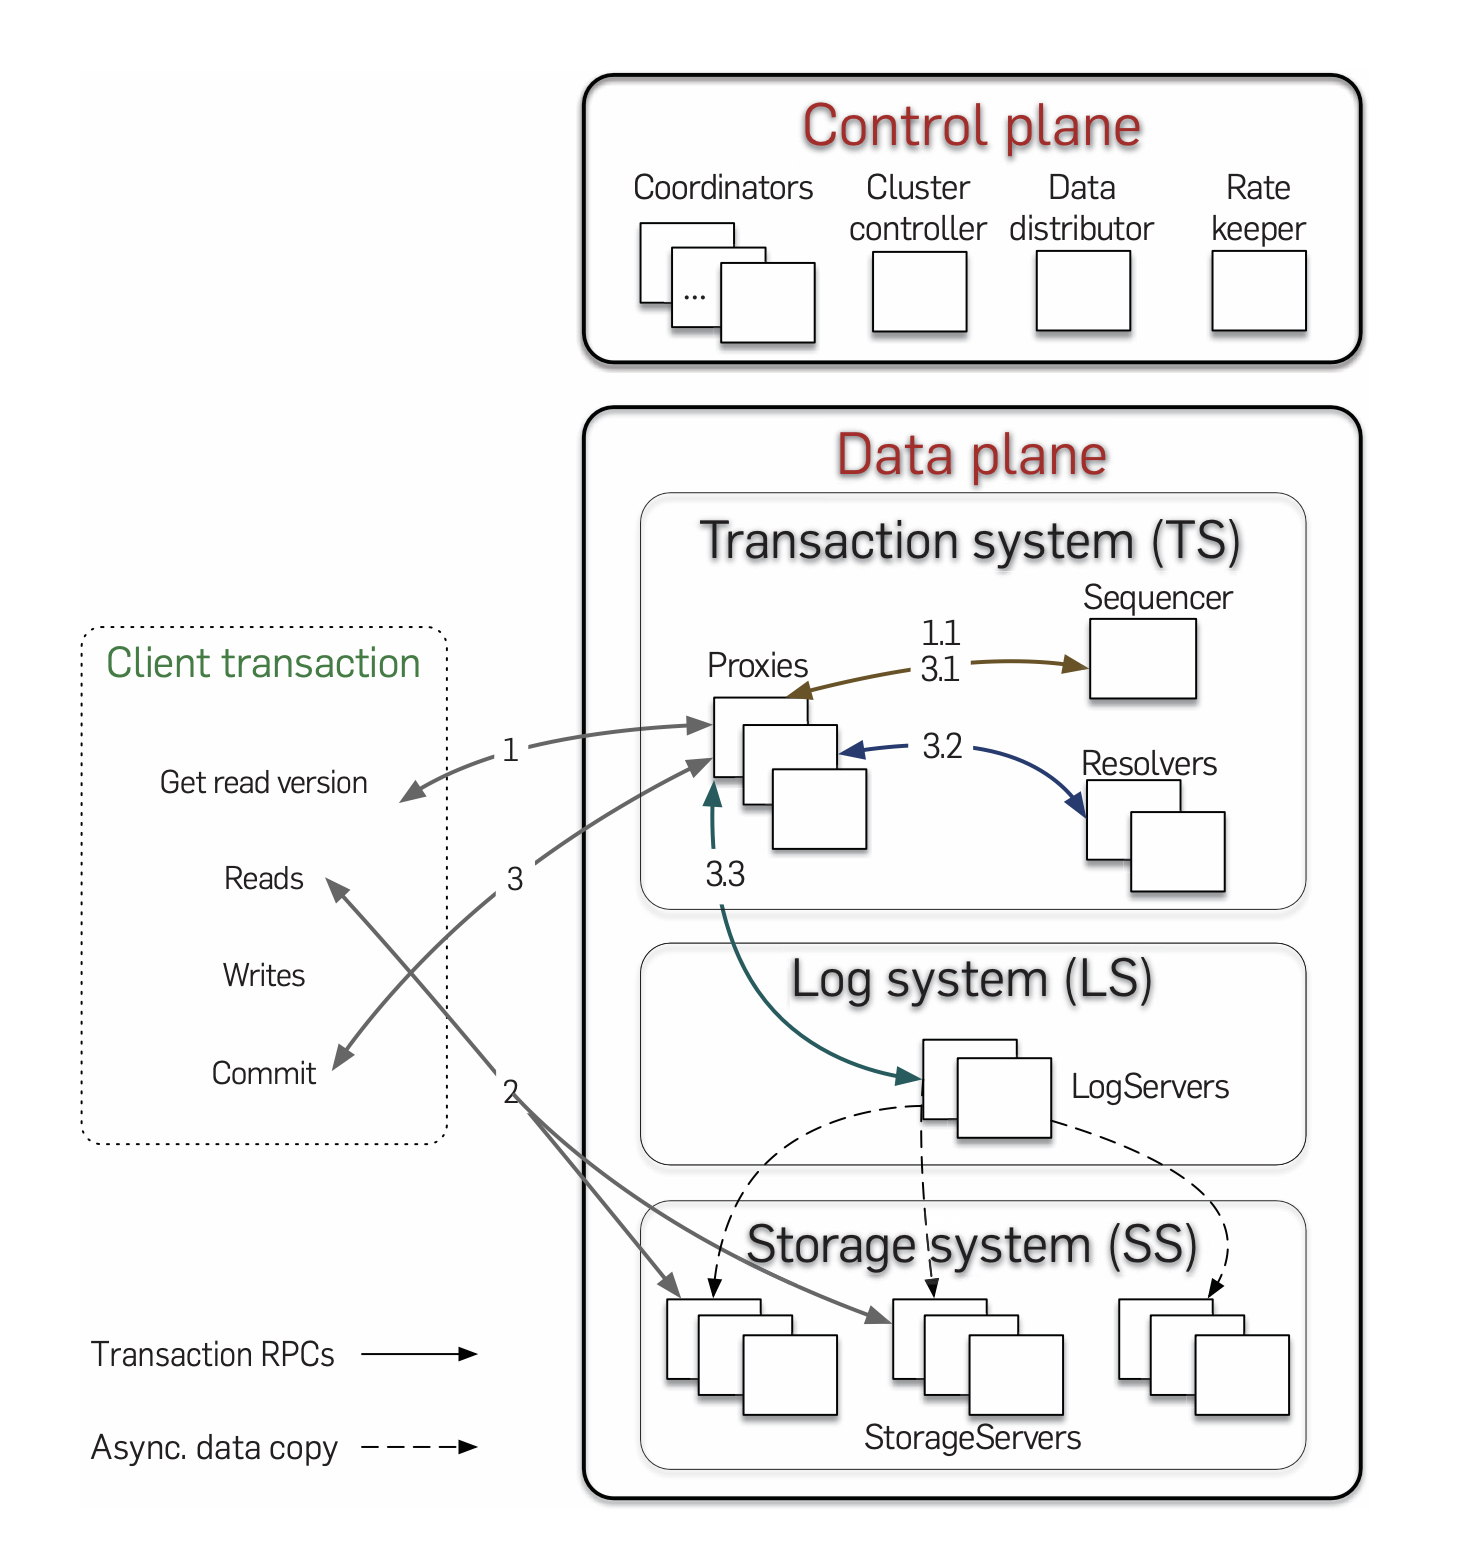
\includegraphics[width=\textwidth]{img/2-Architecture/Architecture and transaction processing.png}
        \end{column}
    \end{columns}
\end{frame}
% %------------------------------------------------
\begin{frame}
    \frametitle{Transactions: Proxy commits P2}
    \begin{columns}
        \begin{column}{0.5\textwidth}
            \begin{enumerate}
    \item Proxy reports the committed version $\rightarrow$ Sequencer, ensures that later transactions' read versions occur after this commit
    \item Proxy replies to the client
            \end{enumerate}
        \end{column}
        \begin{column}{0.5\textwidth}
            \centering
            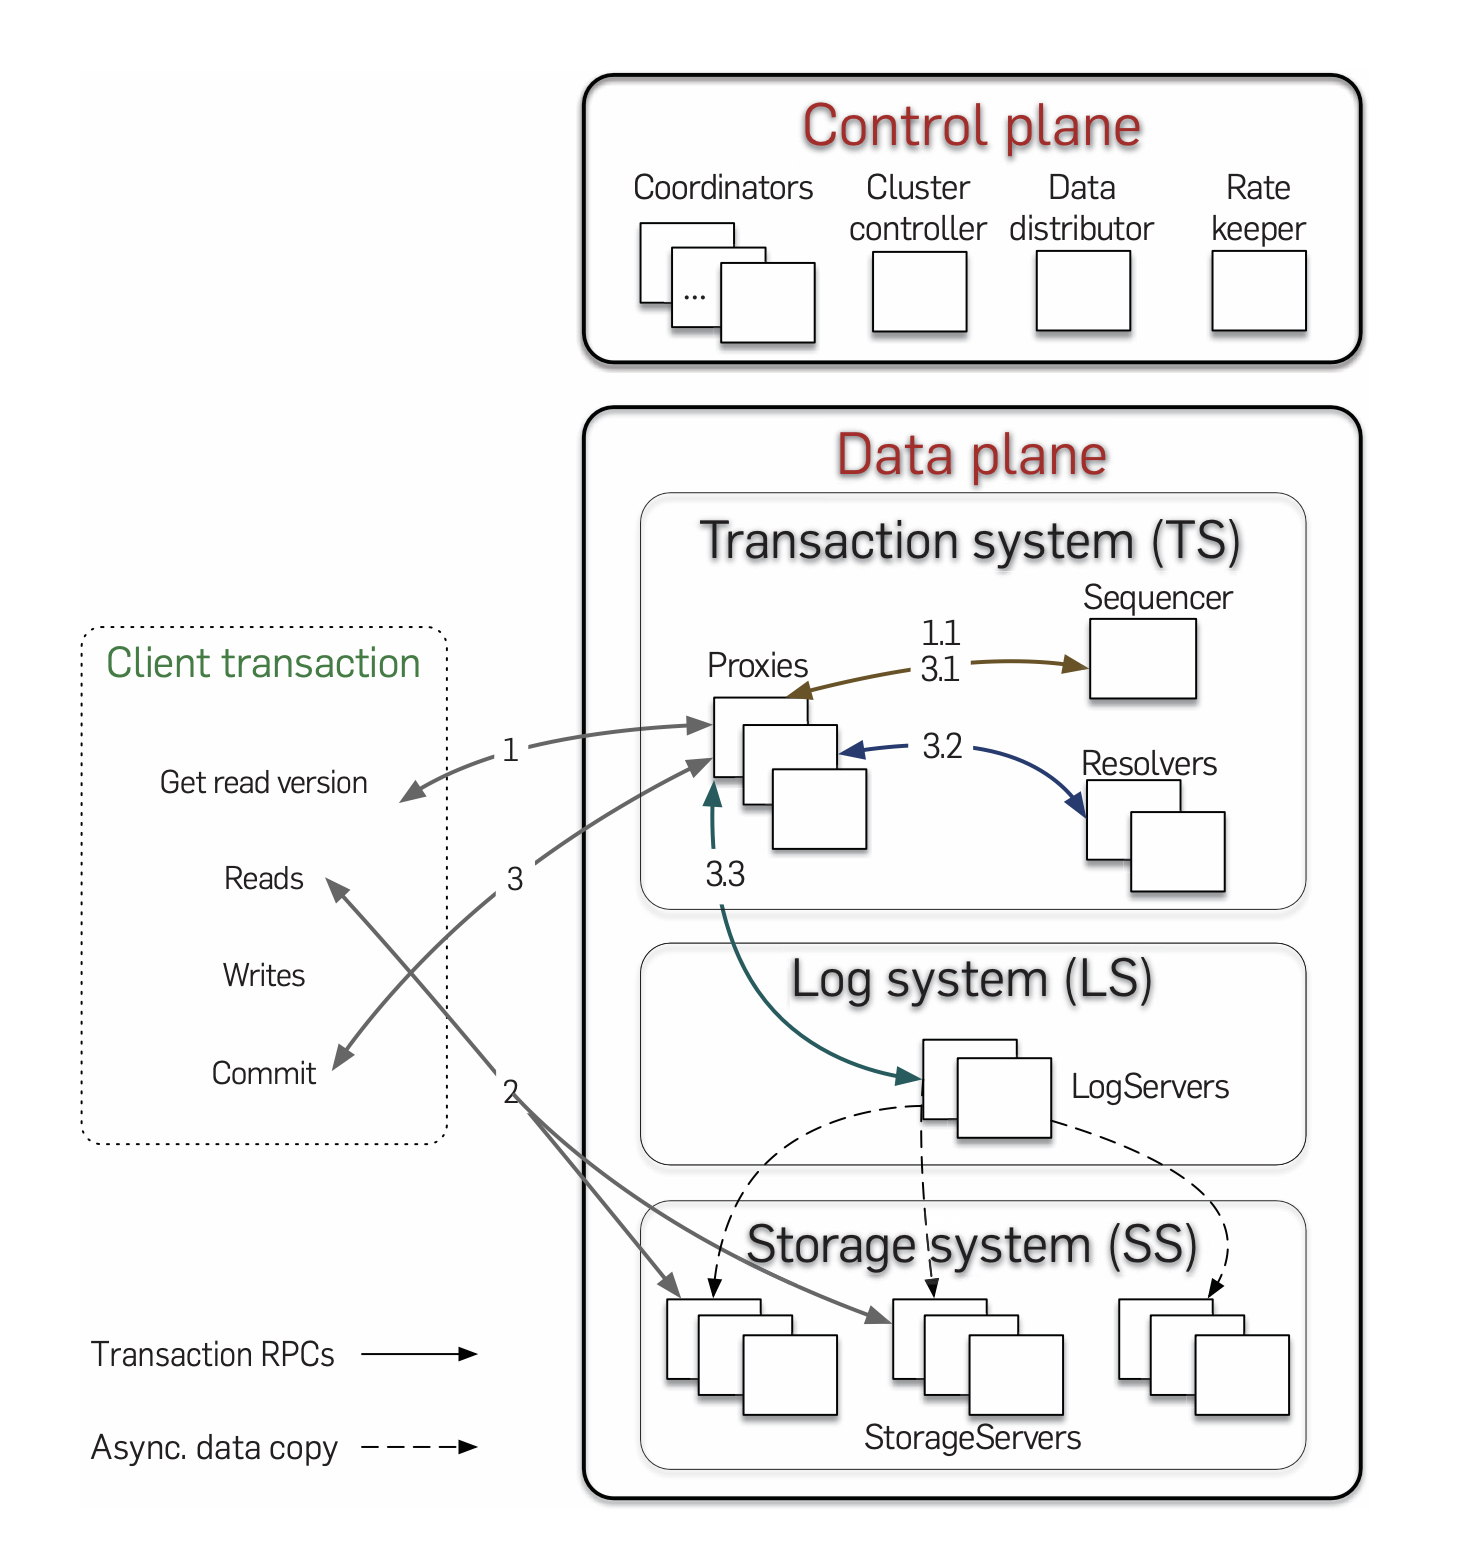
\includegraphics[width=\textwidth]{img/2-Architecture/Architecture and transaction processing.png}
        \end{column}
    \end{columns}
\end{frame}


% %------------------------------------------------


\begin{frame}
	\frametitle{Strict serializability}
\begin{itemize}
  \item FDB ensures strict serializability via Serializable \textbf{Snapshot Isolation} , combining \textbf{OCC} with \textbf{MVCC}.
%   \item Transactions obtain read and commit versions from the Sequencer.
  \item A transaction can commit only when all Resolvers admit the transaction
%   \item The key space is \textbf{divided among Resolvers for parallel conflict detection}.
  \item Optimistic Concurrency Control design \textbf{simplifies TS and SS interactions} but results in \textbf{wasted work for aborted transactions} (client restart the transaction)
\end{itemize}

 \end{frame}


% %------------------------------------------------

\begin{frame}
    \frametitle{Transaction system recover}
    \begin{columns}
        \begin{column}{0.5\textwidth}
            \begin{enumerate}
                \item Traditional databese uses \textbf{ARIES Recovery} (checkpoint, redo, undo).
                \item In FD the recovery is purposely made \textbf{very cheap}, greatly simplifying design choice: \textbf{redo log processing is the same as the normal log forward path}.
                \item System can easily recruit a new TS system in case of failure (Sequencer, Proxies, Resolvers).
            \end{enumerate}
        \end{column}
        \begin{column}{0.5\textwidth}
            \centering
            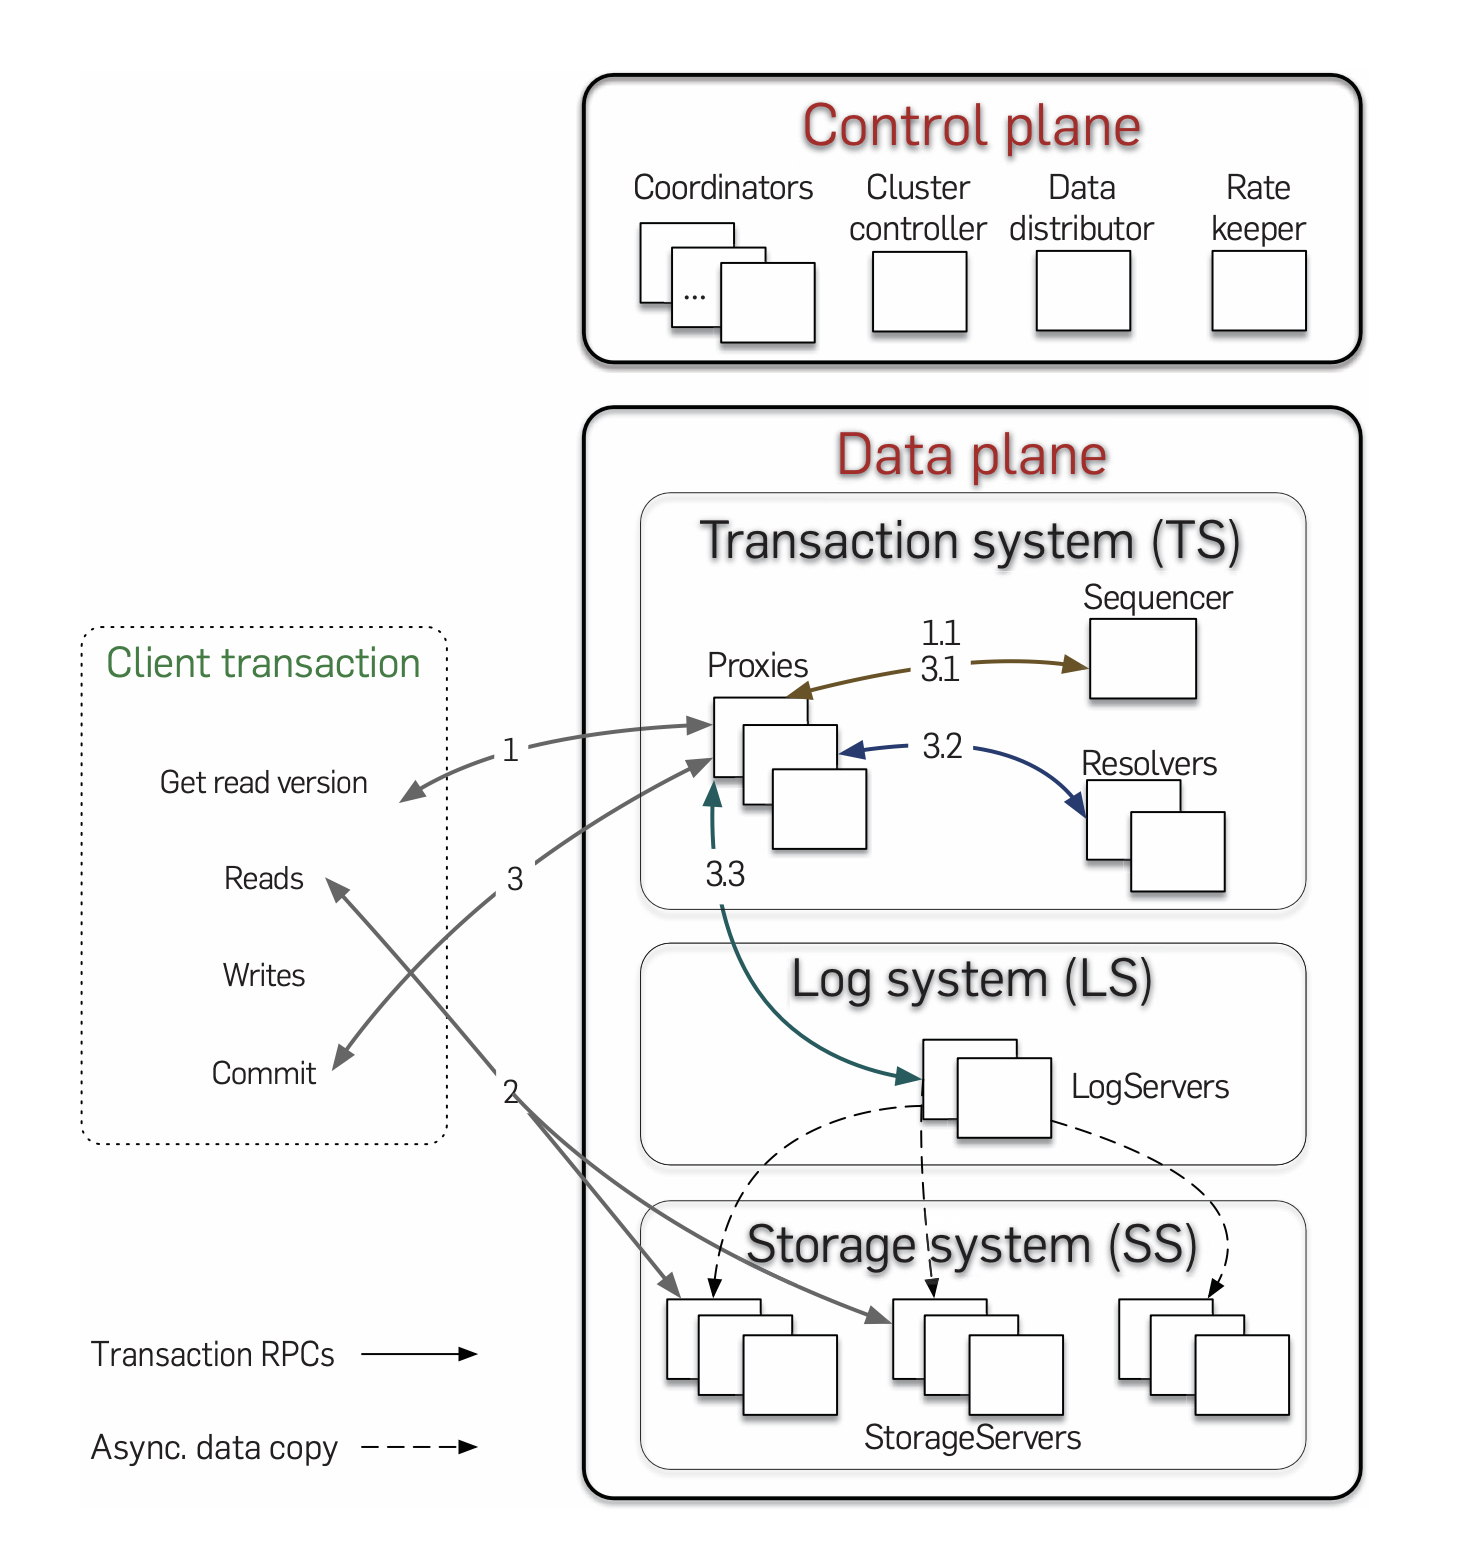
\includegraphics[width=\textwidth]{img/2-Architecture/Architecture and transaction processing.png}
        \end{column}
    \end{columns}
\end{frame}

%------------------------------------------------



% \begin{frame}
% 	\frametitle{Replication: Metadata}
%     \begin{itemize}
%       \item System metadata of the control plane is stored on Coordinators using \textbf{Disk Paxos} (consensus protocol used for reliable data replication across multiple nodes optimized for disk storage)
%       \item As long as a quorum (majority) of Coordinators are live, this metadata can be recovered.

% \end{itemize}
% \end{frame}

 %------------------------------------------------


% \begin{frame}
% 	\frametitle{Replication: Log}
% \begin{itemize}

%       \item When a Proxy writes logs to Log Servers, each sharded log record is synchronously replicated on \textbf{multiple Log Servers}.
%       \item Only when all Log Servers have replied with successful persistence can the Proxy send back the commit response to the client.
%       \item Failure of a Log Server results in \textbf{transaction system recovery}.

% \end{itemize}
% \end{frame}

 %------------------------------------------------


% \begin{frame}
% 	\frametitle{Replication: Storage}
% \begin{itemize}

%       \item Every shard (key range) is asynchronously replicated with multiple Storage Servers, forming a "\textbf{team}".
%       \item A Storage Server usually hosts multiple shards (key range) to evenly \textbf{distribute data across many teams}.
%       \item Failure of a Storage Server triggers Data Distributor to move data from affected teams to healthy ones.

% \end{itemize}
% \end{frame}
\section{Simulation and Testing }

\begin{frame}
    \frametitle{Simulation Testing for Foundation DB}
    \begin{itemize}
        \item Testing and debugging distributed systems is challenging, particularly for Foundation DB.
        \item FDB employs an ambitious approach using a \textbf{deterministic discrete-event simulation}.
        \item The simulation environment quickly exposes bugs in the database, ensuring reproducibility for investigation.
    \end{itemize}
\end{frame}
%------------------------------------------------
\begin{frame}
    \frametitle{Deterministic Simulator}
    \begin{itemize}
        \item All database code is deterministic and multi-threaded concurrency is avoided (instead, one database node is deployed per core).
        \item \textbf{All sources of non determinism and communication are abstracted}, including network, disk, time, and pseudorandom number generator
        \item \textbf{Flow}, a syntactic extension to C++, facilitates deterministic execution of highly concurrent code.
    \end{itemize}
\end{frame}
%------------------------------------------------

\begin{frame}
    \frametitle{Flow, concurrency on C++}
    
\includegraphics[width=2cm]{img/3-Testing/cpp.png}

    \vspace{0.5cm}
   FDB needed to implement efficient asynchronous communicating processes with raw speed and I/O efficiency of C++.
\vspace{0.5cm}

Flow is an extention to the C++ 11 standard that is used to add async/await-like
concurrency primitives with automatic cancellation.

   
\end{frame}

%------------------------------------------------
% \begin{frame}
%     \frametitle{Execution of the Simulator}
%     \begin{itemize}
%         \item Workloads written in Flow interact with simulated FDB servers.
%         \item Multiple FDB servers communicate through a simulated network in a single discrete-event simulation.
%     \end{itemize}
% \end{frame}
%------------------------------------------------

\begin{frame}
    \frametitle{The FDB deterministic simulator}
    \begin{center}
        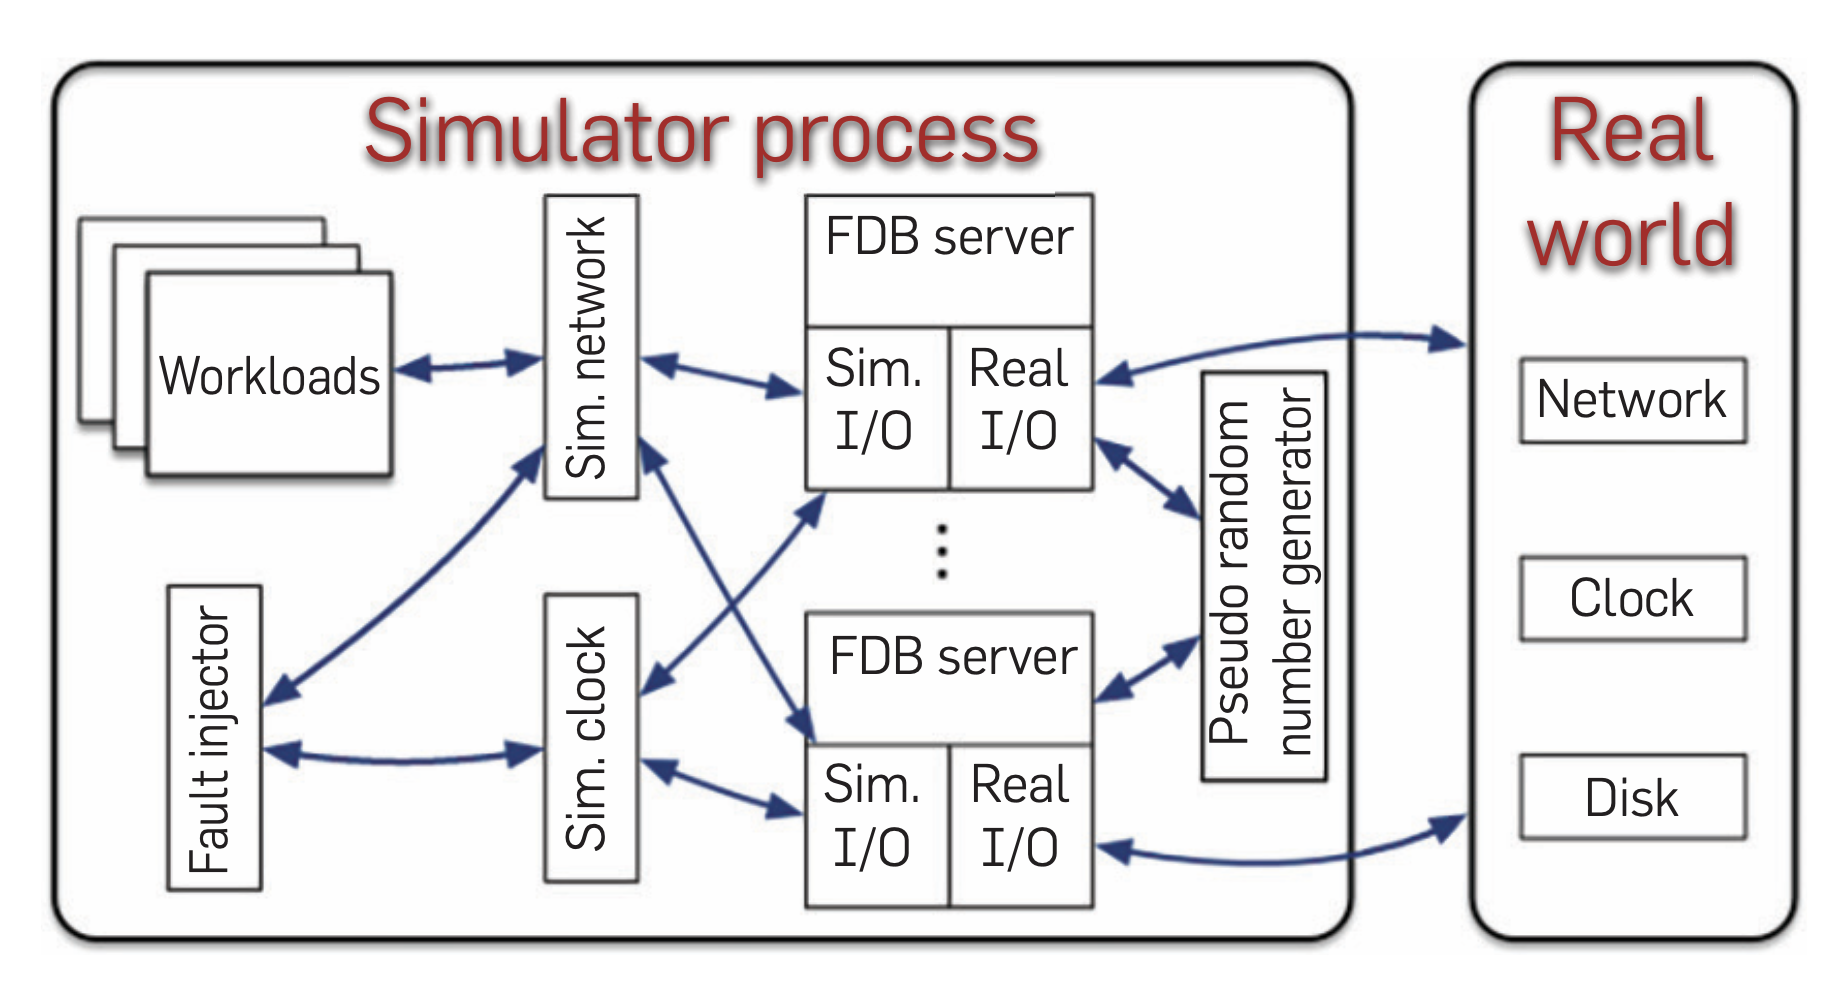
\includegraphics[width=0.8\textwidth]{img/3-Testing/The FDB deterministic simulator.png}
    \end{center}
    
\end{frame}


%------------------------------------------------
\begin{frame}
    \frametitle{Testing the system}
    \begin{itemize}
        \item FDB uses various test to detect failures in simulation.
        \item \textbf{Assertions and invariants} can only be maintained through ATOMIC transaction and isolation.
        \item Recoverability is checked by set of \textbf{failures sufficient to break
the database’s availability}.
    \end{itemize}
\end{frame}
%------------------------------------------------
\begin{frame}
    \frametitle{Fault Injection}
    \begin{itemize}
        \item Simulation injects various faults such as machine failures, network partitions, and disk behavior.
        \item FDB cooperates with the simulation to make rare states and events more common through "\textbf{buggification}"
        \item Maximizes simulation diversity by randomizing cluster size, workloads, fault injection parameters.
    \end{itemize}
\end{frame}


\begin{frame}
    \frametitle{Buggification}
    Simulation is allowed to inject some unusual (\textbf{not contractbreaking}) behavior such as 
    \begin{itemize}
        \item Unnecessarily returning an error from an operation that usually succeeds
        \item Injecting a delay in an operation that is usually fast
        \item Choosing an unusual value for a tuning parameter
    \end{itemize}
\end{frame}
%-------------------------------
\begin{frame}
    \frametitle{Limitations of Simulation}
    \begin{itemize}
        \item Simulation may not reliably detect performance issues or test \textbf{third-party dependencies}.
        \item Simulation cannot reliably detect performance issues, such as an imperfect load-balancing algorithm
    \end{itemize}
\end{frame}
\section{Evaluation of FoundationDB}

\begin{frame}
    \frametitle{Evaluation: Scalability and Performance}
    \begin{itemize}
        \item Conducted on a test cluster of 27 machines in a single data center.
        \item Each machine: 16-core 2.5 GHz Intel Xeon CPU, 256 GB memory, 8 SSD disks.
        \item Configuration: 14 StorageServers on 7 SSD disks, LogServer on remaining SSD.
        \item Synthetic workload: Blind writes, range reads, point reads, and point writes.
        \item Write and read performance evaluated using different transaction types.
    \end{itemize}
\end{frame}
%------------------------------------------------
\begin{frame}
    \frametitle{Throughput and average latency}
    \begin{center}
        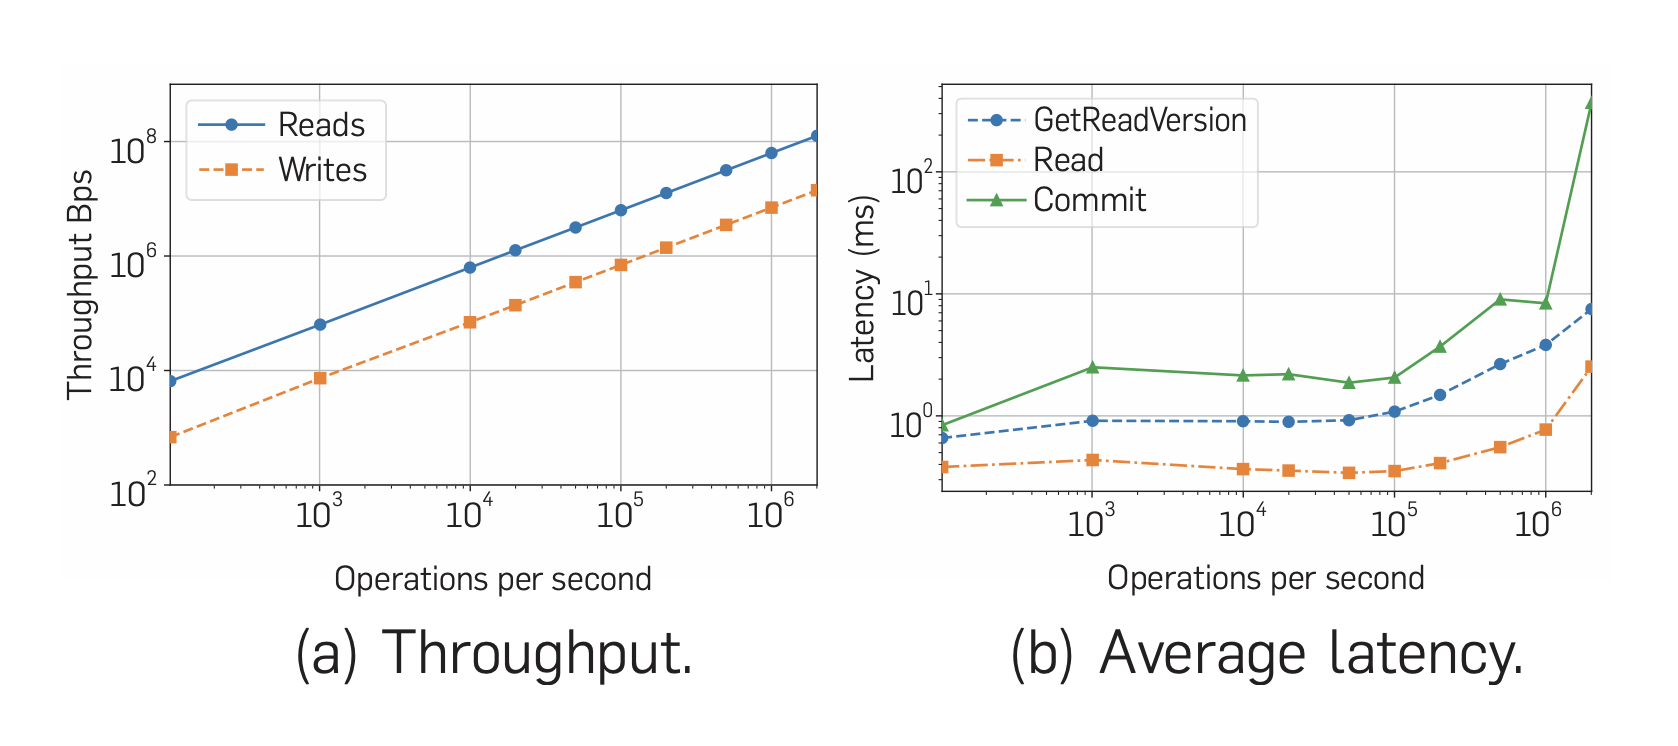
\includegraphics[width=0.8\textwidth]{img/4-Evaluation/Throughput-Average latency.png}
    \end{center}
\end{frame}

\section{Conclusion}

\begin{frame}
    \frametitle{Architecture Design}
    \begin{itemize}
        \item \textbf{Divide-and-conquer} design enables flexible cloud deployment.
        \item Separation of transaction system from storage layer enhances flexibility and scalability.
    \end{itemize}
\end{frame}
%------------------------------------------------
\begin{frame}
    \frametitle{Simulation Testing}
    \begin{itemize}
        \item \textbf{Simulation testing} accelerates bug detection and debugging.
        \item Increased reliability through rigorous correctness testing.
    \end{itemize}
\end{frame}
%------------------------------------------------
\begin{frame}
    \frametitle{Fast Recovery}
    \begin{itemize}
        \item \textbf{Fast recovery} simplifies software upgrades and configuration changes.
        \item Significantly reduces downtime compared to traditional rolling upgrades.
    \end{itemize}
\end{frame}
%------------------------------------------------
\begin{frame}
    \frametitle{5s MVCC Window}
    \begin{itemize}
        \item Choice of \textbf{5-second MVCC} window limits transaction sizes (Storage server keeps recent transaction in memory).
        \item Majority of OLTP use cases are accommodated within this window.
        \item Exceeding the time limit often exposes inefficiencies in client applications.
        \item Transactional tasks can be divided into smaller transactions to fit within the window.
    \end{itemize}
\end{frame}



%----------------------------------------------------------------------------------------
%	CLOSING SLIDE
%----------------------------------------------------------------------------------------

\begin{frame}[plain] % The optional argument 'plain' hides the headline and footline
	\begin{center}
		{\Huge Thanks for your time}
            
	\end{center}
\end{frame}

%----------------------------------------------------------------------------------------

\end{document} 